% ============================================================
% 第 4 章 实验结果
% ============================================================
\section{实验结果}\label{sec:results}

\subsection{总体胜负}\label{sec:wins}

表~\ref{tab:wins} 汇总了四个（生成模型 $\times$ 评委）格子的盲评胜负。在全部 240 对有效比较中，\baseline{} 胜出 224 对（93.3\%），\wordpairs{} 仅胜 15 对（6.3\%），平局 1 对。四个格子的结论高度一致：最“接近”的格子（V4.1-Flash 生成、V4-Pro 评审）中 \wordpairs{} 也仅获 8/60 胜；差距最大的格子（V4-Pro 生成）中 \wordpairs{} 仅 1/60 胜。若剔除唯一平局并做二项符号检验，239 次非平局比较中 \baseline{} 获胜 224 次，显著性远超常规阈值（$p<10^{-40}$）。这与先验概率 0.5 的“无差异”假设形成强烈对比：\textbf{在所考察的开放式生成场景中，词对提示几乎总是降低最终产物的竞争力}。

\begin{table}[htbp]
\centering
\caption{盲评胜负汇总（每格 60 对；行 = 生成模型，列属性 = 评委）}
\label{tab:wins}
\small
\begin{tabular*}{\textwidth}{@{\extracolsep{\fill}} l l r r r r}
\toprule
生成模型 & 评委模型 & \baseline{} 胜 & \wordpairs{} 胜 & 平局 & \wordpairs{} 胜率 \\
\midrule
V4.1-Flash & V4.1-Flash & 54 & 5 & 1 & 8.3\% \\
V4.1-Flash & V4-Pro    & 52 & 8 & 0 & 13.3\% \\
V4-Pro    & V4.1-Flash & 59 & 1 & 0 & 1.7\% \\
V4-Pro    & V4-Pro    & 59 & 1 & 0 & 1.7\% \\
\midrule
\multicolumn{2}{l}{\textbf{合并}} & \textbf{224} & \textbf{15} & \textbf{1} & \textbf{6.3\%} \\
\bottomrule
\end{tabular*}
\end{table}

值得注意的两个跨格子规律。第一，\textbf{生成模型越强，词对提示伤害越大}：V4-Pro 生成时 \wordpairs{} 胜率从 8.3\%--13.3\% 跌至 1.7\%。一个直观解释是：强模型的 \baseline{} 输出本身已具备较高的结构完整性与细节密度，留给前置联想环节的改进空间更小，而词对带来的目标稀释代价不变甚至相对更大。第二，\textbf{交叉评审与自评格子的结论几乎相同}（V4-Pro 生成时，两个评委均给出 59/1/0），未观察到明显的自我增强偏差影响胜负方向的现象。

\subsection{五维平均分}\label{sec:scores}

表~\ref{tab:dims} 报告各格子两条件在五个维度上的平均分，图~\ref{fig:radar} 以雷达图呈现双评委均值。四个格子呈现一致的形态：\baseline{} 在逻辑性、具体性、可操作性与整体质量四个维度全面占优，\wordpairs{} 仅在原创性维度部分反超。以合并配对视角（第 \ref{sec:diff} 节），唯一方向相反的维度正是原创性。

\begin{table}[htbp]
\centering
\caption{五维平均分（10 分制；按生成模型 $\times$ 评委分组，$n=60$/格）}
\label{tab:dims}
\small
\begin{tabular*}{\textwidth}{@{\extracolsep{\fill}} l l l r r r r r}
\toprule
生成模型 & 评委 & 条件 & 逻辑性 & 具体性 & 可操作性 & 原创性 & 整体 \\
\midrule
\multirow{4}{*}{V4.1-Flash} & \multirow{2}{*}{V4.1-Flash} & \baseline{} & 8.97 & 8.87 & 8.78 & 7.53 & 8.88 \\
 &  & \wordpairs{} & 7.95 & 7.40 & 6.88 & \textbf{8.05} & 7.62 \\
\cline{2-8}
 & \multirow{2}{*}{V4-Pro} & \baseline{} & 9.00 & 8.92 & 8.85 & 7.68 & 8.87 \\
 &  & \wordpairs{} & 7.92 & 7.62 & 7.20 & \textbf{8.33} & 7.82 \\
\midrule
\multirow{4}{*}{V4-Pro} & \multirow{2}{*}{V4.1-Flash} & \baseline{} & 8.93 & 8.82 & 8.47 & 7.42 & 8.78 \\
 &  & \wordpairs{} & 6.95 & 6.05 & 5.58 & 7.20 & 6.40 \\
\cline{2-8}
 & \multirow{2}{*}{V4-Pro} & \baseline{} & 9.02 & 9.02 & 8.57 & 7.52 & 8.80 \\
 &  & \wordpairs{} & 6.93 & 6.25 & 5.73 & \textbf{7.82} & 6.62 \\
\bottomrule
\end{tabular*}
\end{table}

\begin{figure}[htbp]
\centering
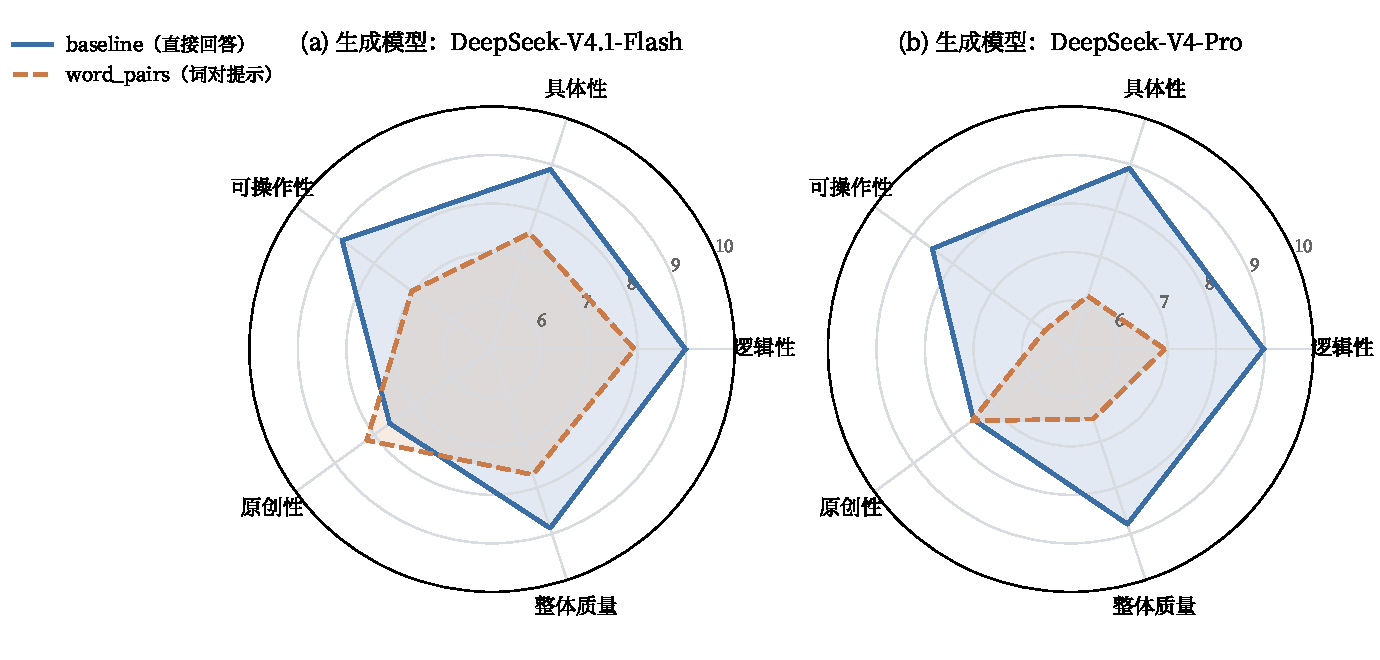
\includegraphics[width=\textwidth]{figs/fig_radar.pdf}
\caption{五维平均分雷达图（双评委均值，10 分制）。虚线（\wordpairs{}）仅在原创性轴超出实线（\baseline{}）。(a) V4.1-Flash 生成；(b) V4-Pro 生成。}
\label{fig:radar}
\end{figure}

维度间的受损幅度存在清晰梯度：受损最重的是\textbf{可操作性}（V4-Pro 生成时低至 5.58--5.73，较 \baseline{} 下降 $2.8\sim2.9$ 分），其次是\textbf{具体性}（下降 $2.8$ 分左右）与\textbf{逻辑性}（下降 $1.0\sim2.1$ 分）。原创性则是唯一出现正增益的维度，且增益幅度（$+0.5\sim+0.7$）明显小于其他维度的损失幅度。这一“原创性小幅增益、其余维度大幅受损”的模式在两个生成模型、两个评委下完全复现，构成了词对提示效果画像的核心。

\subsection{配对分差与显著性检验}\label{sec:diff}

逐对配对分差（式~\eqref{eq:diff}）比格子均值更能刻画分布形态。表~\ref{tab:tests} 报告 240 对合并样本五个维度的分差统计量与两项检验结果；图~\ref{fig:dist} 展示整体质量与原创性两个维度的分差直方图。

\begin{table}[htbp]
\centering
\caption{合并配对分差 $\Delta^{(d)}$ 的统计检验（$n=240$；正值表示 \baseline{} 更优；Wilcoxon 检验剔除零差后进行）}
\label{tab:tests}
\small
\begin{tabular*}{\textwidth}{@{\extracolsep{\fill}} l r r r r r r r}
\toprule
维度 & 均值 & 标准差 & 中位数 & 正/零/负 & $t$ & $p$（配对 $t$） & $p$（Wilcoxon） \\
\midrule
逻辑性   & $+1.54$ & 1.23 & 1 & 204/29/7  & 19.42  & $<10^{-50}$ & $<10^{-34}$ \\
具体性   & $+2.08$ & 1.52 & 2 & 214/14/12 & 21.10  & $<10^{-55}$ & $<10^{-35}$ \\
可操作性 & $+2.32$ & 1.57 & 2 & 220/8/12  & 22.88  & $<10^{-61}$ & $<10^{-37}$ \\
原创性   & $-0.31$ & 1.25 & 0 & 71/62/107 & $-3.88$ & $1.3\times10^{-4}$ & $8.8\times10^{-5}$ \\
整体质量 & $+1.72$ & 1.27 & 2 & 224/1/15  & 21.02  & $<10^{-55}$ & $<10^{-36}$ \\
\bottomrule
\end{tabular*}
\end{table}

\begin{figure}[htbp]
\centering
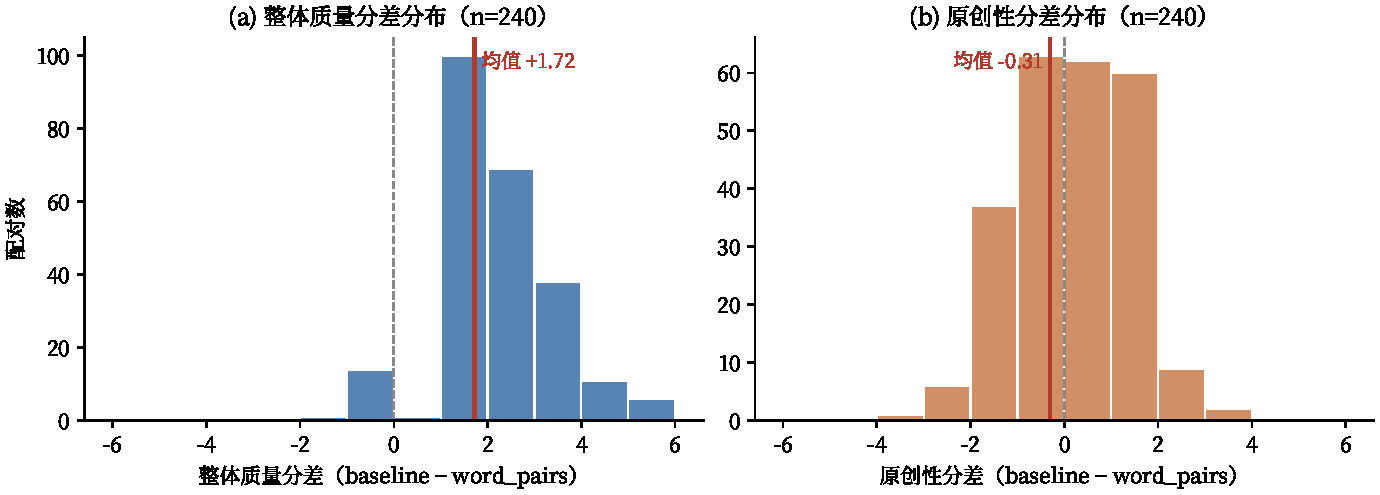
\includegraphics[width=\textwidth]{figs/fig_dist.pdf}
\caption{配对分差分布（$n=240$）。(a) 整体质量分差集中于正值区（均值 $+1.72$）；(b) 原创性分差分布近似对称且略偏负（均值 $-0.31$，即 \wordpairs{} 略优）。}
\label{fig:dist}
\end{figure}

结果有三点值得强调。第一，\textbf{整体质量的差异在统计上极端显著}：配对 $t=21.02$（$p\approx3\times10^{-56}$），Wilcoxon $p\approx4\times10^{-37}$；两项检验基于不同假设得出一致结论，且分差分布（图~\ref{fig:dist}a）并非由少数极端离群对驱动，而是整体右移、中位数为 $+2$。第二，\textbf{原创性维度的反向效应虽小但稳定显著}：均值 $-0.31$（即 \wordpairs{} 平均高 $0.31$ 分），107 对为负、71 对为正、62 对为零（$p\approx8.8\times10^{-5}$）。效应方向与幅度均与胜负分析一致。第三，各维度的零差比例差异揭示了评价行为特征：原创性维度出现 62 次零差（25.8\%），远高于其他维度（3.3\%--12.1\%），说明评委在原创性上的分辨粒度较粗、常给出同分；而整体质量维度仅 1 次零差，因为评委被强制给出胜负结论。

\subsection{任务异质性}\label{sec:tasks-hetero}

图~\ref{fig:task} 按任务分解 \wordpairs{} 的胜场（每柱满分 20，虚线为随机水平 10）。两个模型呈现相同的不均匀格局：\textbf{六个任务中五个任务的词对胜场接近于零}（V4-Pro 生成时 T1--T4、T6 全部为 0/20），唯一例外是 \textbf{T5 人格模型}——V4.1-Flash 生成时获得 7/20 胜，虽仍未过半，却远高于其余五个任务的 1--2/20（Fisher 精确检验 $p=1.2\times10^{-3}$）；V4-Pro 生成时也仅在 T5 获得胜场（2/20）。合并双模型后，T5 贡献了全部 15 场胜局中的 9 场（$p=1.0\times10^{-4}$），是词对策略唯一具有实质竞争力的任务。

\begin{figure}[htbp]
\centering
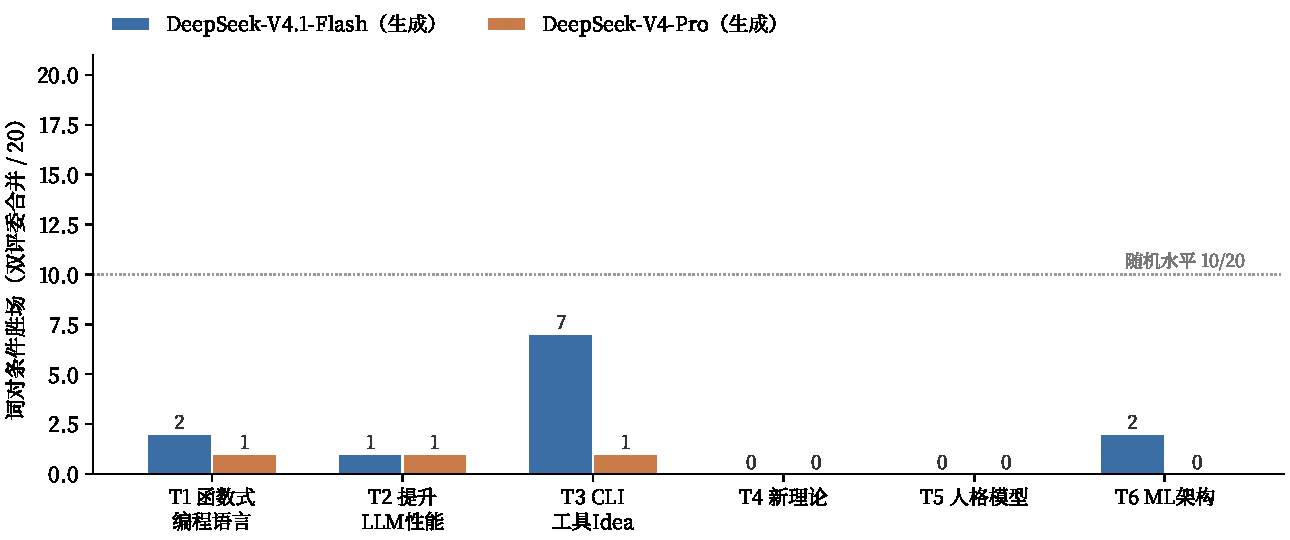
\includegraphics[width=0.92\textwidth]{figs/fig_task.pdf}
\caption{按任务分解的 \wordpairs{} 胜场（双评委合并，每柱满分 20）。虚线为 50\% 随机水平。T5（人格模型）的胜场远高于其余任务，贡献全部 15 胜中的 9 胜。}
\label{fig:task}
\end{figure}

T5 的特殊性可以从任务性质解释。人格模型设计（“提出一个新的类似于九型和荣格八维的模型”）是一个\textbf{概念构建型}任务：产出的核心价值在于提出一套自洽、有辨识度的分类学隐喻（轴、相、枢、介质等），而非工程可落地性；且该领域存在九型人格、MBTI、荣格八维等大量先例，模型的 \baseline{} 输出容易落入既有框架（评委理由中多次出现“更像成熟模型的组合”），原创性天花板受限。词对联想恰好在该任务上补足了短板：随机意象（潮汐、编织、光谱）为分类学提供了新鲜的命名与结构隐喻。这与第 \ref{sec:scores} 节“原创性是唯一受益维度”的发现互相印证：\textbf{词对提示的价值集中在“新颖性本身即核心价值”的任务上}。相反，T1/T3/T6 等工程方案类任务对可行性、技术细节的要求刚性更强，联想词无法弥补细节密度的损失。

\subsection{生成与清洗成本}\label{sec:cost}

词对提示不仅损失质量，还显著增加成本（表~\ref{tab:cost}、图~\ref{fig:cost}）。生成 token 方面，V4.1-Flash 的 \wordpairs{} 条件平均消耗 8252 个完成 token，是 \baseline{}（4089）的 \textbf{2.02 倍}；V4-Pro 为 1.60 倍（9796 对 6123）。耗时方面分别为 1.57 倍（37.5 s 对 23.9 s）与 1.36 倍（119.9 s 对 88.1 s）。清洗阶段进一步引入成本：清洗调用本身消耗 token，且词对输出中有 57\%--64\% 的字符（词对列表与相关引用）被剥离——V4.1-Flash 的压缩比为 0.43，V4-Pro 为 0.36。

\begin{table}[htbp]
\centering
\caption{生成与清洗成本（均值 $\pm$ 标准差；长度为字符数；压缩比 = 清洗后/原始长度）}
\label{tab:cost}
\small
\begin{tabular*}{\textwidth}{@{\extracolsep{\fill}} l l r r r r}
\toprule
生成模型 & 条件 & 完成token & 耗时/s & 输出长度 & 清洗后长度（压缩比） \\
\midrule
\multirow{2}{*}{V4.1-Flash} & \baseline{}   & $4090\pm2520$ & $23.9\pm12.5$ & $2774\pm1302$ & --- \\
 & \wordpairs{} & $8252\pm2767$ & $37.5\pm12.5$ & $4319\pm1100$ & $1960\pm$（0.43） \\
\midrule
\multirow{2}{*}{V4-Pro} & \baseline{}     & $6123\pm3396$ & $88.1\pm42.3$ & $3576\pm1652$ & --- \\
 & \wordpairs{} & $9796\pm2956$ & $119.9\pm48.6$ & $4090\pm1148$ & $1588\pm$（0.36） \\
\bottomrule
\end{tabular*}
\end{table}

\begin{figure}[htbp]
\centering
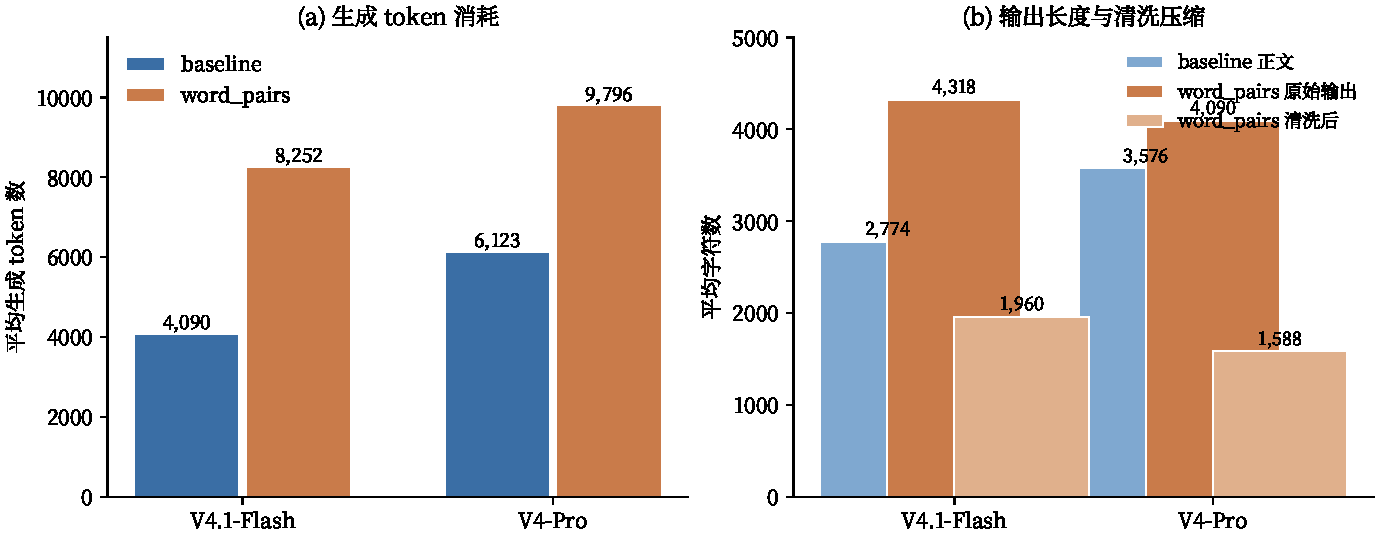
\includegraphics[width=\textwidth]{figs/fig_cost.pdf}
\caption{生成与清洗成本对比。(a) 平均完成 token 数：\wordpairs{} 条件为 \baseline{} 的 1.60--2.02 倍；(b) 输出长度与清洗压缩：清洗后的词对正文（浅色）反而短于 \baseline{} 正文。}
\label{fig:cost}
\end{figure}

最值得关注的发现是\textbf{长度反转}：词对条件的原始输出更长（字符数 4090--4319 对 2774--3576），但剥离词对与引用后，其正文长度（1588--1960）反而\textbf{显著短于} \baseline{} 正文——V4-Pro 生成时仅为 \baseline{} 的 44\%。换言之，词对提示把生成长度预算的过半数消耗在了被丢弃的过程性内容上，正文的信息密度与展开程度双降。这也部分解释了具体性与可操作性的大幅受损：在上下文长度与生成预算双重受限下，词对列表直接挤占了正文的技术细节空间。

\subsection{位置偏差分析}\label{sec:position}

表~\ref{tab:position} 报告 A/B 位置偏差。四个格子中三个出现 A 位均值高于 B 位（差值 $+0.16\sim+0.58$ 分），一个格子相反（$-0.18$ 分），平均 A 位优势约 $+0.27$ 分，量级远小于条件主效应（$+1.72$ 分）。条件化分差显示了两面性：当 \baseline{} 位于 A 位时 A$-$B 分差（$+1.42\sim+2.77$）大于 \wordpairs{} 位于 A 位时的分差绝对值（$-0.59\sim-2.14$），提示 A 位优势与条件效应存在部分叠加，可能使观测到的 \baseline{} 胜率略有高估。但即便在最保守的估计下（假设位置效应完全单向叠加），其幅度（$<0.6$ 分）也不足以解释 $93.3\%$ 的胜率与 $+1.72$ 的整体分差；且位置已由确定性哈希平衡，两组条件在 A 位的比例接近对半，位置偏差对两条件是对称的。综上，\textbf{位置偏差不改变本研究的方向性结论}。

\begin{table}[htbp]
\centering
\caption{评委位置偏差（A/B 位平均分与条件化分差）}
\label{tab:position}
\small
\begin{tabular*}{\textwidth}{@{\extracolsep{\fill}} l l r r r r}
\toprule
生成模型 & 评委 & $\bar S_A$ & $\bar S_B$ & \shortstack{A$-$B 分差\\（A 位为 \baseline{}）} & \shortstack{A$-$B 分差\\（A 位为 \wordpairs{}）} \\
\midrule
V4.1-Flash & V4.1-Flash & 8.33 & 8.17 & $+1.65$ & $-0.97$ \\
V4.1-Flash & V4-Pro    & 8.60 & 8.08 & $+1.42$ & $-0.59$ \\
V4-Pro     & V4.1-Flash & 7.50 & 7.68 & $+2.75$ & $-2.14$ \\
V4-Pro     & V4-Pro    & 8.00 & 7.42 & $+2.77$ & $-1.60$ \\
\bottomrule
\end{tabular*}
\end{table}

\subsection{与前版实验的对比}

本实验（v2）是同一研究问题第二版协议的执行结果，前版（v1）使用单一生成模型（Kimi-K3，经 NVIDIA NIM 端点）且清洗协议较弱。表~\ref{tab:v1} 汇总两版结果：v1 中 \baseline{} 胜 49/60，但 17/60 的清洗样本残留词对引用，其“\baseline{} 大幅占优”的结论存在混淆——残留引用可能被评委当作幻觉。v2 将清洗残留降为 0，并引入双生成模型、双评委与位置哈希平衡，\baseline{} 胜率反而\textbf{上升}至 93.3\%。这说明 v1 的结论并非清洗伪影所致：在彻底消除残留引用、且评委被明确告知“引用本身不扣分”的条件下，词对条件的整体劣势依然存在甚至更加清晰。两版实验在原创性维度上也一致（v1：7.15 对 8.25；v2：词对略优），进一步支持了该方向性发现。

\begin{table}[htbp]
\centering
\caption{与前版实验（v1）的协议与结果对比}
\label{tab:v1}
\small
\begin{tabular*}{\textwidth}{@{\extracolsep{\fill}} l l l}
\toprule
项目 & v1 & v2（本文） \\
\midrule
生成模型 & Kimi-K3（单模型） & V4.1-Flash + V4-Pro \\
评委 & 同一生成模型（单一） & 两个模型交叉（各评一次） \\
有效比较数 & 60 & 240 \\
清洗残留 & 17/60 & \textbf{0/120} \\
位置平衡 & 随机交换 & 确定性哈希平衡 \\
\baseline{} : \wordpairs{} : 平 & 49 : 10 : 1 & 224 : 15 : 1 \\
\bottomrule
\end{tabular*}
\end{table}
